\documentclass{acm_proc_article-sp}

\usepackage {subfigure}

\def\eg{{\it e.g.,\/}}
\def\ie{{\it i.e.,\/}}
\def\etal{{\it et al.\/}}


\begin{document}

\title{Object-oriented vs Event-based middleware}
%\subtitle{[Abstract]}


\numberofauthors{4} 
\author{
\alignauthor
Satarupa Mukherjee \\
       \affaddr{University of Alberta}\\
       \email{satarupa@ualberta.ca}
\alignauthor
Eric Luong \\
       \affaddr{University of Alberta}\\
       \email{eluong@ualberta.ca}
\and  
\alignauthor 
Todd Mortimer \\
       \affaddr{University of Alberta}\\
       \email{rmortime@ualberta.ca}
\alignauthor 
Timo Ewalds\\
      \affaddr{University of Alberta}\\
       \email{tewalds@ualberta.ca}
}


\maketitle
\begin{abstract}

In this survey, we compare object oriented middleware and event based middleware with an emphasis on applications for each middleware type. We identify time, space and synchronization coupling as three distinguishing criteria between middleware implementations, and use these criteria to identify why particular applications are more or less well suited to particular middleware platforms. Using these criteria, we identify that object and event based systems have complementary characteristics that make one middleware type more suitable where the other is less so. 

\end{abstract}

%%%%%%%%%%%%%%%%%%%%%%%%%%%%%%%%%%%%%%

\section{Introduction}
\label{sec:intro}

%[first page]

Middleware provides a common interface through which distributed applications and systems can interact. Depending on the application requirements, this interaction can be as simple as basic message passing or as complex as distributed state synchronization. Between these extremes, applications take on a spectrum of functional requirements that drive the corresponding middleware requirements. While some applications may be highly time sensitive, others may be latency tolerant. Some applications may be required to scale to hundreds or thousands of interacting entities, while others require tight coupling between a small number of hosts. Different middleware solutions possess a range of capabilities as diverse as this set of application requirements, providing the developer with a spectrum of choice when considering which middleware platform is best suited to their application.

In this survey, we examine the technical and practical aspects of both object oriented and event based middleware. We discuss the characteristics and some technical implementations of each type, and find that both event based and object oriented systems each follow their own basic set of functional semantics but vary widely in terms of technical details. We identify time, space and synchronization coupling as three basic criteria by which different middleware systems are distinguished, and cast both object oriented and event based systems into where they typically fall within this set of criteria. Using these three distinguishing criteria as a guide, we discuss several applications of both object oriented and event based middleware systems. We find that these systems each have their own strengths and weaknesses, and are especially well suited or poorly suited to different applications in complementary ways.

This survey proceeds as follows: Section \ref{sec:technical} provides a general overview of both object oriented and event based middleware. We introduce the three distinguishing criteria of time, space and synchronization coupling in Section \ref{sec:timespace}, and discuss how these criteria can identify which applications are more or less appropriate for different middleware implementations in Section \ref{sec:apps}. We conclude in Section \ref{sec:conclusion}.



%%%%%%%%%%%%%%%%%%%%%%%%%%%%%%%%%%%%%%

\section{Technical Overview}
\label{sec:technical}
%[half page]

% different purposes
% different centricities
% spectrum in all cases

In this section we will briefly review some of the technical details on both object oriented and event based middleware systems. While we will see that both object oriented middleware and event based middleware exist within a spectrum of technical implementation details, each middleware type typically follows a common procedural semantic through which entities interact. 

Object and event based systems are rooted in different functional requirements, which subsequently inform their technical implementations. Object oriented middleware has its roots in Remote Procedure Calls, and is therefore typically concerned with the correct coordination of activity between remote entities. Event or message based systems evolved from the simple requirement for different entities to exchange information and are less concerned about whether or not the different entities are acting in concert. Thus, object middleware is typically functionality-centric, while event based middleware tends to be data-centric. These different centres of interest are reflected in the technical capabilities of each system type. 

In the following subsections, we briefly discuss the technical implementations and characteristics of  object oriented middleware, followed by event based systems. 

% CORBA as all things to all people - does OO and events - makes a mess of it?



%%%%%%%%%%%%%%%%%%%%%%%%%%%%%%%%%%%%%%

\subsection{Object-Oriented Middleware}
\label{sec:techobj}
%[one page]

%[How does it work, principles]

As software systems became distributed, Remote Procedure Calls (RPCs) were developed to facilitate communication between separate applications that need not be located on the same machine.  As described in Vivnoksi \etal\ \cite{Vinoski:2004p8371}, client applications are able to utilize procedures on server applications with RPCs in the same way that they would call local procedures.  RPCs generally hide the fact that operations are happening in a distributed fashion, making calls to local procedures and remote procedures look the same to the programmer.

RPCs evolved into Object-oriented middleware (OOM) and gained the benefit of object-oriented concepts such as inheritance, encapsulation, polymorphism, object references and exceptions \cite{Pinus:2006p8367,Vinoski:2004p8371}.  As many of today's most popular languages are object-oriented, OOM fits in naturally and allows developers to work within a familiar environment.

OOM uses distributed objects to coordinate processes on multiple hosts.  A distributed system based on OOM is made up of several types of components.  The most prominent two components are the client application and the server-side object.  The middleware serves to allow the client to communicate with the object on the server.  This is typically accomplished through code that is generated by the middleware itself.  A stub object is created on the client side to facilitate communication between the client and the server.  It provides the interface to the server-side object for the client's use and it takes care of network communication details, such as the marshalling of parameters and unmarshalling of a received response.  Similarly, a skeleton object is created on the server side for the same purpose in reverse, unmarshalling the parameters of the invocation and marshalling the response.  The stub and the skeleton work on top of the middleware core.

%[DIAGRAM HERE, or after the paragraph that follows.  It should be a simple diagram of the process, either in implementation or in general.  Possible candidates include Figure 5 of Emmerich's paper (CORBA.pdf), Figure 2.1 of the ICE manual, the diagram on the Java RMI wikipedia page, or this lovely diagram (except they use the terms "caller" and "called object" instead of "client" and "server side object"): http://en.wikipedia.org/wiki/File:Distributed_object_communication.png ]

\begin{figure}
\centering
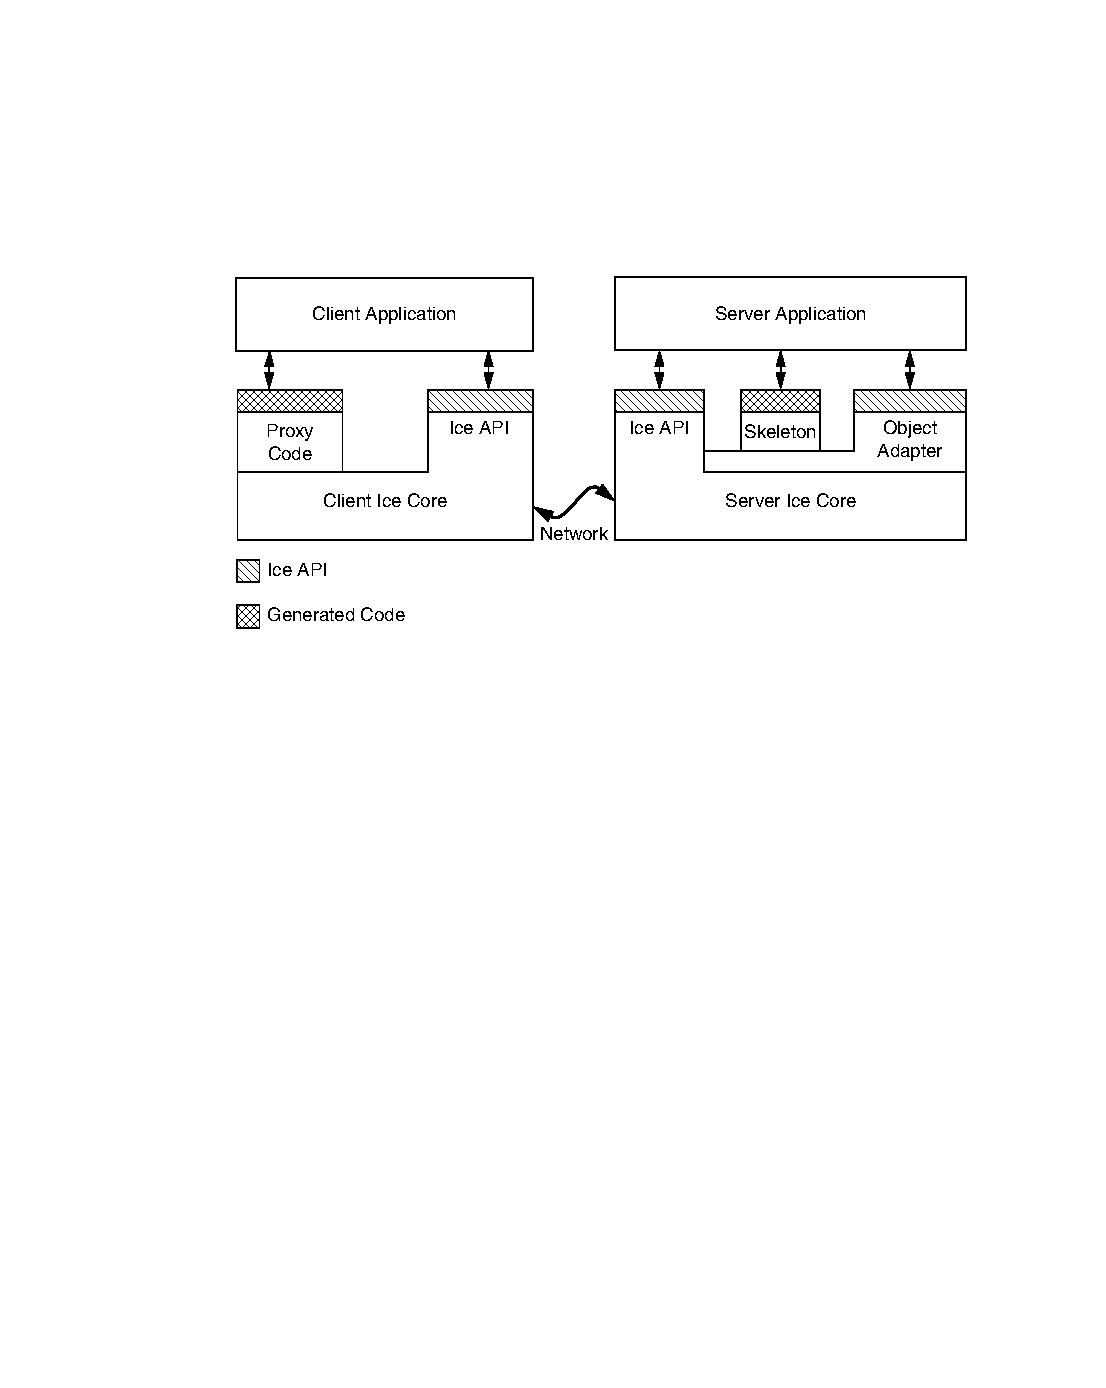
\includegraphics[width=8cm]{icefig21.pdf}
\caption{Components involved in Object Requests, from \cite{icemanual}}
\label{fig:icefig21}
\end{figure}

The general process within this architecture is as follows:
\begin{description}
\item[Client Invocation] The client initiates communication by calling a method on the stub object.
\item[Network Request] The client stub marshalls the request information and sends it over the network to the server.
\item[Server Execution] The server-side skeleton receives and unmarshalls the request.  It then performs the appropriate action on the server-side object.
\item[Network Response] If there is a return value, this value is passed back to the skeleton.  The skeleton marshalls the information and sends it back over the network.
\item[Invocation Completion] The client stub receives the results, unmarshalls the data and returns it to the caller.
\end{description}

Figure \ref{fig:icefig21} shows how the Internet Communications Engine (ICE), developed by ZeroC, implements this architecture and process.

%The client initiates communication by calling a method on the stub object.  The stub takes care of marshalling the request information and sends it over the network to the server, where it is received by the skeleton object.  The skeleton unmarshalls the request and performs the appropriate action on the server-side object.  If there is a return value, this value is passed back to the skeleton.  The skeleton marshalls the information and sends it back to the client stub, which unmarshalls it and returns the value to the calling client.  This process is illustrated in Figure \ref{fig:icefig21}.

%%%%% I used "citation needed" below, which should probably be resolved with some random throwaway papers.  Or we can just not cite for those points (in which case we should probably remove the citation for CORBA as well).

This architecture is followed by most, if not all, of the major OOM systems in use, including the Common Object Request Broker Architecture (CORBA) developed by the Object Management Group (OMG) \cite{Emmerich:2007p8368}, Java's Remote Method Invocation (RMI) \cite{Vinoski:2004p8371} and Microsoft's Distributed Component Object Model (DCOM) \cite{Pinus:2006p8367}.  Specific implementation of this stub-skeleton architecture varies by system.  As already mentioned, ICE also follows this architecture.  However, their client stubs are called "proxies" instead \cite{icemanual}.  This overview of the architecture is also simplified - depending on the system, communication may also be facilitated by other components such as object request brokers (ORBs) and object adapters.

A client must have a way of finding the location of the server, even if it is mostly taken care of by the middleware.  Object references are bound to server address information.  Binding may be direct or indirect.  In direct binding, object references know the address of the server endpoint itself, whereas indirectly bound references use the location of an implementation repository or lookup service which can then be used to find the location of the server itself \cite{Henning:2004p8372}.  Indirect binding is more expensive, but also more flexible.  Servers can be migrated easily since the object references will remain valid \cite{icemanual}.

As with RPCs, OOMs tend to hide the distributed nature of an application and seek to provide transparency.  For example, suppose that a client object has a proxy to an object on the server.  As far as the client is concerned, the object is local.  The proxy provides method stubs that can be used by the client and, when called, the stubs initiate the network request and take care of all of the work necessary for network communication.  When the server object finishes its work, a response is sent back in the same way.  In most cases, this entire process is hidden from the client.

The communication described above is synchronous, though some OOMs will offer asynchronous communication methods as well.  For example, ICE allows for both asynchronous invocation and asynchronous call dispatch \cite{Henning:2004p8372}.  Invocation is how the client calls the server, and dispatch is how the server responds to the client.  In asynchronous invocation, the server is given a callback object from the client.  The callback object is used to return the results of the invocation asynchronously.  By using asynchronous invocation, the client does not need to wait for the invocation to complete, but can access the return value when it is needed later.  The server-side will not be able to distinguish between synchronous or asynchronous invocation on the client side; it functions the same way in either case.  Asynchronous call dispatch works the other way around.  When the server receives an invocation, it can set it aside without tying up an execution thread.  A response can be delivered later on (in ICE, by invoking a callback function).  The client will not know whether the server is using synchronous or asynchronous dispatch.

As Vinoski notes in \cite{Vinoski:2004p8371}, distributed systems are becoming increasingly heterogeneous.  A network may consist of many different types of machines which are running different operating systems and using different software.  The network composition continues to change as time passes, and it can be difficult for distributed processes to operate over a network that is heterogeneous and inherently dynamic.  Middleware in general helps to solve this problem.  However, the distributed process may be heterogeneous itself.  The distributed objects that are part of the process may be written in different programming languages such as C, C++ and Java.  To deal with this problem, many OOMs (including CORBA, ICE and DCOM) offer an Interface Definition Language (IDL).  An IDL describes the different constructs that make up the middleware's object model.  Different middleware systems use different IDLs.  CORBA uses the OMG IDL whereas ICE uses the Specification Language for ICE (SLICE) \cite{Henning:2004p8372}.  DCOM uses its own Microsoft IDL.  Java RMI does not have an IDL - it only allows communication between Java objects.  An IDL can be mapped to corresponding objects within different programming languages, thereby allowing objects written in different languages to communicate with each other over the middleware, provided that the appropriate language mappings are available.

% This section probably needs a firmer conclusion...



%%%%%%%%%%%%%%%%%%%%%%%%%%%%%%%%%%%%%%

\subsection{Event Based Middleware}
\label{sec:techeb}
%[one page]

Event based middleware (EBM) systems are often alternately referred to as Message Oriented Middleware (MOM) or Publish / Subscribe (PubSub) systems, but they all follow the same basic semantics. In EBM systems, entities are typically broken down into producers and consumers. The producers generate events and send them to the consumers, who receive and react to them. The mechanics of how these systems function vary within a wide range, but the functional semantics are typically broken down into three phases:

\begin{description}
\item[Advertisement] The producer indicates what kinds of events or messages they can produce.
\item[Registration] Consumers choose one or many advertisements and indicate what events they would like to be notified of.
\item[Notification] The producers begin sending events to the interested consumers.
\end{description}

\begin{figure}[hbt]
\centering
\begin{minipage}{6.0cm}
\subfigure[Direct Communication]{
	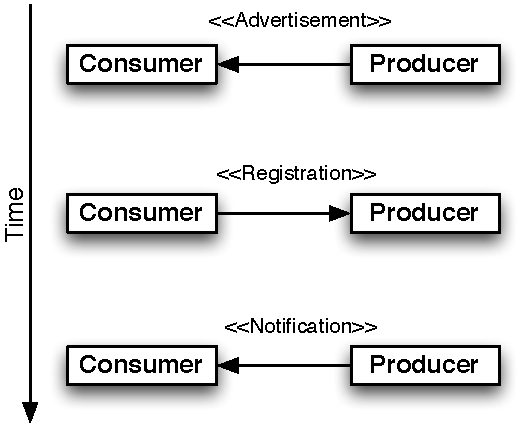
\includegraphics[width=6.0cm]{ebbasic.pdf}
	\label{fig:ebbasic}
}
\end{minipage}
\begin{minipage}{8.0cm}
\subfigure[Brokered Communication]{
	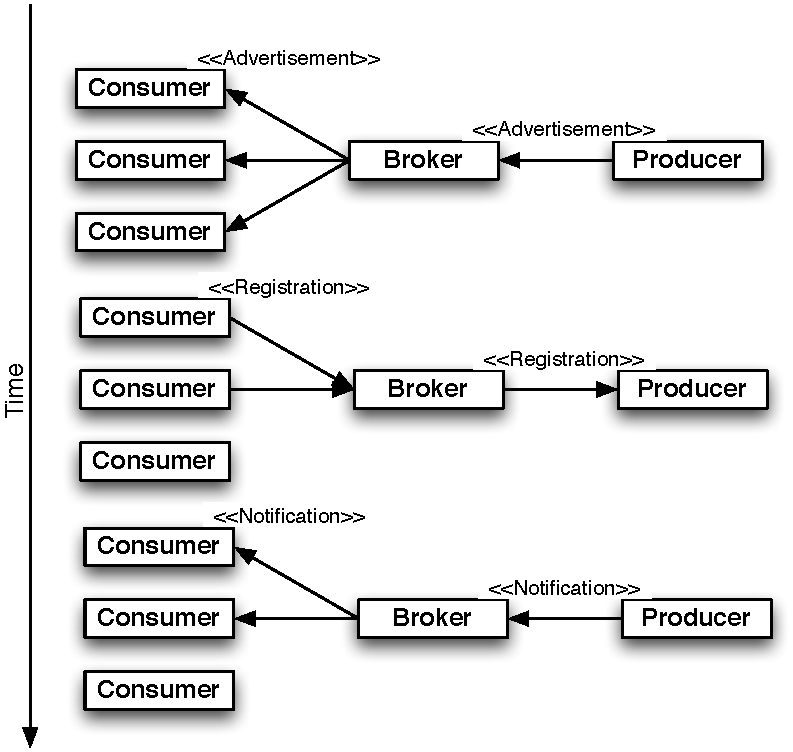
\includegraphics[width=8.0cm]{ebbroker.pdf}
	\label{fig:ebbroker}
}
\end{minipage}
\centering
\caption{Functional Semantics of Event Based Middleware}
\label{fig:ebsemantics}
\end{figure}


Each of these phases can have different levels of abstraction which subsequently inform the qualities of the system. In some systems, the advertisement phase is absent completely and consumers must discover event producers through some other mechanism. For example, in a tightly coupled system such as system event notifications on a single host - such as Microsoft's COM+ Events system or the Mac OS X Notification system - information about which event producers are available and which events they produce may simply be listed in programmer documentation. Alternately, the Cambridge Event Architecture (CAE) includes a facility for event producers to be directly queried by consumers for lists of which events they produce and the interface for subscribing to those events \cite{Bacon:2000p6818}. In this system, consumers interact directly with producers to both discover and subscribe to events, and notifications are then delivered directly to those consumers by the producer. This is depicted in Figure \ref{fig:ebbasic}. If we introduce a layer of indirection between the producer and consumer, as in Figure \ref{fig:ebbroker}, an intermediate service may act as a broker between producers and consumers. In this type of system, consumers interact with the broker as they would with the producer directly, and the producer communicates only with the broker. In this way, the producer sends its advertisements to the broker, who then makes those advertisements available to consumers. For example, in the PADRES system multiple brokers form a network through which advertisements are flooded, \cite{Jacobsen:2010p8313}, eventually reaching all the consumers in the system.

Registration and Notification phases can be handled similarly. The consumers can register with the event producer directly, such as in CAE \cite{Bacon:2000p6818}, or they can register with some intermediate entity, such as a broker. Typically, if a consumer registers with a broker then they will also receive notifications through the same broker. While the direct registration and notification system is simpler to conceptualize and build, the layer of abstraction provided by the brokered architecture has advantages for scaling and performance, as the burden of communicating with consumers is moved from the producer to the broker. This performance and scalability concern is significant enough that some event architectures which are primarily designed with direct communications between producers and consumers in mind, such as CAE \cite{Bacon:2000p6818} and Java Message Service (JMS) \cite{Oracle:2002p8432}, have extensions which introduce brokers between consumers and producers and can be leveraged to improve performance on heavily loaded systems.

In addition to different design choices for the mechanics of event advertisement, registration and notification, there is a similar range of choices for the implementation of the events or messages themselves. In tightly coupled systems, messages can be serialized platform specific objects passed between producer and consumer, such as serialized Java Beans in JMS \cite{Oracle:2002p8432}, or objects defined by the programmer through an IDL, such as in CORBA Events \cite{Siegel:1999p8569}. In these instances, some level of system homogeneity is required, in that both producer and consumer must understand object formats and semantics. More loosely coupled systems implement messages as specially formatted strings of ordinary text, and a producer or consumer simply has to understand the format of messages in order to participate in the system. PADRES is an example of such a system where entities interact by passing textual messages to each other \cite{Jacobsen:2010p8313}, and messages simply consist of lists of parameter values formatted into tuples (\ie\ [Param, =, Value]).

In addition to a spectrum of message formats, there is a spectrum of registration types. In the simplest registration systems, consumers simply register for all events of some type and subsequently receive notifications of all such events. The CORBA Event Service is like this, in that consumers subscribe to some event channel and subsequently receive every event that is posted to that channel . In more complex systems, clients can subscribe to some subset of events by supplying a filter. Filters typically specify some range of event parameter values that the consumer is interested in, and producers or brokers refrain from passing events that do not match that filter to those clients. Most event based middleware supports this kind of filtering, including JMS, CORBA Notifications, CAE and PADRES. More complex still is the composition of events into composite event registrations, in which a consumer registers for an event which is composed of two or more other events. Support for this kind of composite registration is less common, and is complicated if the consumer registers for composite events which are supplied by different producers. CAE and PADRES both support composite event registrations through their brokers, who handle the business of registering for the individual event notifications and then perform the event composition for the consumer. The difference between the two implementations is in the nature of the composing entity: In CAE the Composite Event Service is monolithic and fixed, whereas in PADRES composite events can be processed by any broker in the network and the brokers work together to choose some broker that can perform the event composition with minimal cost in terms of network resources and broker computation resources. In this way, the PADRES composite event implementation scales better than the CAE implementation.

We see then that there is a wide spectrum of event based middleware. System semantics typically follow the Advertise $\rightarrow$ Register $\rightarrow$ Notify paradigm, but the details of how each of these phases works can vary between implementations. Communications between consumers and producers can be direct or mediated by brokers, with resultant effects on performance and scalability. Events and messages themselves can be implemented in both platform dependent or platform independent ways, and the mechanism for achieving platform independence can be either through some shared specification, such as when IDLs are used, or simply through the use of plain text messages which are parsed by system entities. Finally, event registrations or subscriptions can range from the simplistic type where all events produced are simply consumed, to the more sophisticated type where events can be filtered out based on consumer preferences, to the very complex where events from different producers can be composed together by system intermediaries and delivered to consumers who have registered for these composite events. While we have largely confined ourselves here to the JMS, CAE, CORBA and PADRES implementations of event or message based middleware, there exist many more implementations, some of which are surveyed by Tarkoma \etal\ in \cite{Tarkoma:2006p6862}.

%Despite their fundamental differences in interest, both object oriented and event based systems are variations on inter-entity communication mechanisms, and can be tooled for similar purposes. As will be seen in the following discussion, CORBA appears as both object oriented and event based middleware. This is because the CORBA Events system is a variation on the original CORBA object middleware \cite{Siegel:1999p8569,Emmerich:2007p8368} which allows CORBA Components to publish event objects which are subsequently consumed by subscribers. In this way, CORBA enables object oriented communication semantics simultaneously with event based communication semantics, at the cost of increased complexity.


%%%%%%%%%%%%%%%%%%%%%%%%%%%%%%%%%%%%%%

\section{Time, Space and Synchronization}
\label{sec:timespace}

While middleware generally enables transparent interaction between systems, the implementation details vary in several ways. One of the significant distinctions between categories of middleware is how the endpoints are coupled. The main three ways that the endpoints can be coupled are in time, space and synchronization \cite{Eugster:2003p6725}. Highly coupled systems appear to be local and are easier to reason about, but are generally not highly scalable. Decoupling can be achieved along these three axes:

\begin{description}
\item[Time Decoupling] The endpoints need not be available at the same time. Messages can be buffered in the middleware and received at a later time, even if the sender is no longer available.
\item[Space Decoupling] The endpoints need not know who is sending or receiving the messages. There may even be multiple senders or receivers for a single message.
\item[Synchronization Decoupling] The endpoints need not wait for each other to process the messages or send a response. If a response is needed, an event or callback will happen when the response arrives.
\end{description}

Given these definitions, we analyze where object-oriented and event-based middleware fit into the spectrum.

Object-oriented Middleware and Remote Procedure Calls generally attempt to disguise the fact that it is a remote call, so must be coupled in time and be synchronous just as a local object or procedure would be. An error will occur if the other endpoint is unavailable or if it is very slow to reply. Most Object-oriented middleware would be considered coupled in space, though some object-oriented middleware use a lookup service to establish a connection with the other endpoint. In these cases the sender and receiver would be partially coupled because they still communicate directly, but use an intermediary to initially locate one another. When sending an asynchronous notification, the middleware would be considered partially synchronous. The sender need not wait for the receiver, but the receiver usually processes the message immediately.  Some object-oriented middleware, such as ICE, allow both asynchronous method invocation and asynchronous call dispatch.  The sender need not wait for the receiver and the receiver may delay execution of the request.  Therefore object-oriented middleware must be coupled in time and tends to be coupled in space, but may actually operate asynchronously in certain implementations.

Many event-based middleware implementations attempt to be fully decoupled for maximum scalability. Some event-based middleware, such as CAE, are only partially decoupled in time and space while enforcing synchronization decoupling, but many of them introduce a broker to allow full decoupling. The broker can buffer messages locally to enable message delivery when either the sender or the intended receiver is offline at the time the message is produced or consumed. In this way, brokers enable producers and consumers to be decoupled in time. Decoupling in space is achieved since the broker delivers messages to all interested parties, allowing the publisher to be oblivious to the identity or number of recipients. Scalability from space decoupling is achieved when there are many interested recipients for a particular message, in which case the broker - or broker network - can typically distribute the message more efficiently than if the publisher had to send the message to each recipient directly. Finally, event based systems are decoupled in synchronization - meaning they are asynchronous - by their nature. This characteristic is made obvious if we imagine what a synchronous event based system would be like: In such a system the event consumer would expect to receive an event notification at the time of subscription, which runs counter to the notion of event systems as notification of when events occur, not when a consumer becomes interested in them. From this discussion, we see that event based middleware is typically decoupled in all three of time, space and synchronization. 

%aka. Buffered / Direct / [A]Synchronous

%[one page]

% 
% I mean the whole middleware thing is defined by whether they are coupled by space, time and synchronization, and who gets the messages. Object oriented is just a group of points in those coordinates, event-based is some other group of points, pub/sub is another set of points
% 
% If we set it up with discussions of obj and the bag of eb middleware, then we can lead into the discussion of the time / space / sync question, and then distinguish what we've already discussed in those terms. We could even talk about applications matching points in that space, which makes them more or less appropriate for different systems
% 
% I think it is good to start with what is expected (Objects here, Events there) and then pull out the spectrum synthesis later
% 
% then we'll discuss applications and how the apps we see fit into the spectrum
% and then why the application coordinates are close to the system coordinates
% 
% Hmm, how would you define event-based middleware? Is the defining point that it is 1:n, or that it is async? or something else?
%
% for me, the defining characteristics are data-centricity and async
% 1:n is a byproduct of the fact that its data centric and not object / host centric
% in an obj system, there's only one object that you talk to (that provides some service or whatever), and you need it to do something. data centric services make distribution to multiple interested parties natural
% 
% I'm trying to figure out the defining points of each of these
%
% what defines object middleware and what defines event middleware?
%
% yeah
% 
% 
% can you explain your three axis to me? I want to put it into an email to the others to give context to the changes / synthesis. I think they'll be happy, because it's a nice package
% so time, space, sync.
% 
% what do you mean by time?
% 
% time essentially means the two machines that are interacting don't need to be even online at the same time. The messages are buffered in the middleware.
% 
% okay. space?
% 
% the two machines don't need to know about each other, they interact by something other than direct references but instead by interest
% 
% okay. and sync?
% 
% synchronization means the machines never block waiting on a response from the other
% the only one that's a little fuzzy is space, but we just have to be clear about what we're talking about. 
% 
% do you think there are any other axis? 
% 
% well, he also defines the axis of interest, but I'm not sure those are orthogonal to the previously defined axis
% 
% nah, I would argue that interest isn't in the same system. Interest is what the system is, time/space/sync is how the system is. object system have interests the same as event systems. they just work differently. that's what discovery services are for
% 
% are these three orthogonal?
% 
% I would say.. can you have x>0 on one and y=z=0 on the others? can we hold sync and space constant while varying time?
% 
% that would effectively just be a really slow connection
% you can be sync, in that you wait until the other guy comes back online
% 
% It may be easier to think of these as buffered, direct and sync
% 
% you can be buffered and direct, in the sense that you know who your end point is, but not have a direct link
% 
% I suppose you could also think of this as where do you put your layer of abstraction.
% 
% that's pretty much what the whole course is about...
% 
% This is a start:
% buffer | direct | sync
% false  | false  | false => fire and forget, only to online hosts : irc
% false  | false  | true  => 
% false  | true   | false => corba notifications
% false  | true   | true  => RPC
% true   | false  | false => event based messages : PADRES
% true   | false  | true  => useless? wait forever
% true   | true   | false => must be buffered locally, distributed event-based
% true   | true   | true  => very slow RPC


%%%%%%%%%%%%%%%%%%%%%%%%%%%%%%%%%%%%%%

\section{Applications}
\label{sec:apps}

Having discussed the dimensions in which middleware systems are decoupled, and what characteristics follow from which decouplings, we now present a discussion of practical applications of both object oriented and event based middleware systems. For each of these applications, we will show how the functional requirements of the application place it at some coordinate in the three axis system of time, space and synchronization decoupling. Given this placement, which kind of middleware is appropriate for the application becomes obvious, and we therefore show that the application requirements are suited to the middleware characteristics. 

After presenting several examples of middleware applications, we discuss which kinds of applications are best suited to both object-oriented and event-based middleware, and which kinds of applications are poorly suited. We will see that each kind of middleware has strengths and weaknesses which are typically the inverse of the other, making object-oriented and event-based middleware complementary. 

\subsection{Object Oriented Middleware}
\label{sec:appsobj}
%[one page for object applications, how they fit in the spectrum]

Object oriented middleware is best suited for applications that are tightly coupled in time and are usually better for applications that require synchronous communication because not all platforms support both asynchronous invocation and asynchronous dispatch.  As we usually consider object oriented middlewares as at least partially coupled in space, they are also better suited for such applications.  Object oriented middlewares are thus best suited for applications that tend to be tightly coupled, rather than those that are loosely coupled.

Object oriented middleware can be used for networking purposes. Denault \etal\ \cite{Denault:2008p8364} discuss an object oriented network middleware used for multiplayer games. In these types of games, players collaborate (or compete) within a graphical world. Each player controls a character known as an avatar. This character is meant for performing actions that usually involve interacting or communicating with objects within the world, other player characters or the world itself (i.e. navigation and travelling). To maintain the notion among players that they are sharing a common location in the game world, each player must have an up-to-date local copy of the game state.  As the state of the world changes (usually due to player actions), each player's local game state must be updated accordingly, in order to maintain consistency among the players.  If consistency is not maintained, the notion of a shared world is lost.

Traditional multiplayer games are short and involve a relatively few number of participants. Denault \etal\ \cite{Denault:2008p8364} assert that such games usually have a maximum of 16 players in any one instance. Massive multiplayer online games (MMOG) do not fit either of these two descriptions.  There may be thousands of players in an instance of the game, and the world is persistent rather than short-lived since the game state is maintained even as different players join and leave the game. The system must therefore be able to handle a large number of connected players, making scalability an important factor in the design of an MMOG. A middleware seeking to support a MMOG would preferably be flexible, distributed, efficient and scalable.  Denault \etal\ \cite{Denault:2008p8364} specifically argue that "\emph{objects} can implement an ideal interface between the game logic and the communication middleware." The authors also state that objects are useful for distribution and state replication.

We have already mentioned the issue of scalability.  With a high number of concurrent users that are located throughout the world, network connection quality has high variability.  Scalability is a key factor in addressing networking issues such as high latency, limited bandwidth and the limitations of individual machines (\ie\ nodes) in the network.  Besides scalability, there are a few other issues that a middleware solution must address.  Consistency is a problem that occurs due to the distributed nature of a MMOG.  Player actions within the game are expected to occur in real time, which means that the player's local game state must be current and synchronized with other players' local states.  If the states do not match then the players are not interacting in the "same" world.  It is important to note that a game world, and thus the representation of the game state, can be extremely large, so much so that storing the entire game state locally is not a feasible solution.  However, an individual player does not require an up-to-date representation of the entire world.  The player is only concerned with the state of the world in his or her vicinity.  Only a subset of the state must be maintained for each player, so that the relevant parts of the world are provided in real-time to the player.  Unfortunately, every player is continuously affecting and modifying the game world.  This fact and the problem of latency in the network together ensure that game state can never be completely up-to-date.  The goal is thus to maintain consistency within a small threshold of tolerance.  A third issue is reliability, which comes into play because MMOGs necessarily mean operation over a large distributed network.  The probability of a node failing increases as the network becomes larger.  As the number of participants in a multiplayer game is very high, the probability of failure will be quite high as well.  Inevitably, nodes will fail and connections will break.  The system must be robust against such problems within the network, handling node and connection failures in a manner that minimizes negative impact on gameplay.

From these challenges, we can identify the location of MMOGs within the coordinate system described in Section \ref{sec:timespace}.  An individual node is concerned with the portion of the game state that is relevant to one particular player.  If the node is unavailable, it means that the player is offline and need not receive any updates.  Time decoupling is therefore unnecessary; it is acceptable that endpoints must be online at the same time for communication to occur.  As the game state is affected by player actions, changes must be communicated to all players.  In most cases, the source of a change need not be known.  In order words, the system may be loosely coupled in space.  Finally, receiving endpoints are expected to process incoming information as quickly as possible in order to maintain as consistent a game state as possible between players.  MMOGs are thus partially synchronous.  It is not fully synchronous because senders need not wait for a response.

Keeping these challenges in mind, the authors have designed an object-oriented middleware composed of four layers: the Game Layer, the Duplicated Objects Layer, the Communication Abstraction Layer and the Network Layer.  The Game Layer maintains the \emph{game objects} that together make up the game state.  These objects naturally model objects within the game world, include players and game items.  Game objects are mapped to \emph{duplicated objects} within the Duplicated Objects Layer.  The Communication Abstraction Layer provides means by which the Duplicated Objects Layer can communicate with other nodes.  Finally, the Network Layer handles the low-level implementation details to facilitate communication and connection establishment.  Duplication objects and the situations in which the Communication Abstraction Layer is necessary are discussed in greater detail in \cite{Denault:2008p8364}.  Interestingly, the Communication Abstraction Layer uses both Remote Method Invocation (RMI) and a publish/subscribe communication abstraction, depending on the situation.  The latter abstraction deviates from traditional object-oriented middleware.

%%%%%%%% Next two paragraphs omitted so as not to go over 10 pages.  Above paragraph was modified to account for this loss.

% Duplicated objects are the units that are distributed among the players so that they have a consistent game state.  Player nodes keep a local instance of these objects, which the authors of the paper call a \emph{duplica}.  Certain player actions can be performed using the duplica only; the authors use the example of a \emph{read} operation on a game object.  Unfortunately, duplica cannot be used for \emph{modifying} operations as doing so allows for the possibility of obvious inconsistency issues.  The authors' example is a game where two players attempt to pick up the same object.  If duplica are used, both could potentially see success (if the other player's success is not communicated in time).  To solve this problem, modifying operations must be sequentially executed on the node that has the duplica deemed to be the \emph{duplication master}.  All other duplica are updated based on changes to the master.

% The Duplicated Objects Layer must communicate to nodes when the when the Game Layer invokes a modifying operation on a duplica.  Reliable, synchronous messaging in the form of Remote Method Invocation (RMI) is used to communicate the change to the duplicate master.  When the master object has significantly changed, all duplicas must be updated to the current state of the master.  Note here that the authors have implemented techniques to determine when change is significant.  They choose not to update duplicas for every little change in order to minimize costly network traffic.  Interestingly, the architecture deviates here from traditional object-oriented middleware.  The authors decided to use a publish/subscribe communication abstraction to keep duplicas up-to-date.

Denault \etal\ \cite{Denault:2008p8364} describe two implementations of this object-oriented MMOG middleware: Mammoth, which is a framework built for academia, and Net-Z, which is a commercial product by Quazal.  The authors conclude with some experiments to test scalability and the effectiveness of different Communication Abstraction Layer implementations. Their conclusions make it is clear that object-oriented middleware is well suited for MMOG development.



%%%%%%% Wrote this while falling asleep - someone please check for dumb mistakes.

As described in Dipper \etal\ \cite{Dipper:2004p8366}, object oriented middlewares have proven to be quite useful in the design of astronomical instrumentation.  Instrument Control System (ICS) software is extremely complex, demanding a great deal of cost and effort  in its implementation and maintenance.  An ICS facilitates the control of an astronomical instrument, and a system may involve the coordination of multiple instruments.  The design of ICS software faces numerous challenges.  As a consequence of legacy systems and international collaboration in ICS development (wherein standards and protocols are not consistent among all parties), control systems in astronomical instrumentation are distributed and usually heterogeneous.  There are also many common requirements between the ICS for different instruments, as well as to some non-astronomical systems.

The authors in \cite{Dipper:2004p8366} suggest that object-oriented middleware is excellent for addressing the above challenges.  Object-oriented middleware means the use of object-oriented design, which enables advantageous techniques such as encapsulation of common function.  Object-oriented practices allow developers to abstract away certain complexities.  In addition, they promote reusability.  The authors find object-oriented middlewares favourable mostly due to these positive consequences of object-oriented design.    The authors describe a particular situation in which their decision to use object-oriented middleware (CORBA) proved beneficial in the development of their new ICS software.  Their software would have to communicate with two other systems that only offered outdated interfaces.  The solution was to use object-oriented middleware to create proxy objects for the two ICS systems.  They also note that these proxies could be easily converted to actual objects to facilitate the conversion of the older systems to an object-oriented middleware.

While, Dipper \etal\ do not provide specific information as to the coupling requirements of ICS software, the nature of the problem suggests that there is tight coupling in space.  ICS are specific to different astronomical instruments, so the identity of sender and receiver is likely to be very important in any communication.  Ultimately, however, the authors did not advocate object-oriented middleware in the domain of astronomical ICS because of these properties, but because of the advantages of object-oriented practices which, for example, promote the reusability of components.  Development of ICS software is extremely time consuming and OO principles  contribute to a relatively rapid development cycle.

Object-oriented middleware has also been used for applications in robotics \cite{Mohamed:2011p8374} and location-aware systems \cite{Jarvensivu:2004p8369}, but discussion on these are omitted for brevity.  As we have seen, one of the major advantages of object-oriented middleware is the natural use of object-oriented design principles.  It is therefore useful for many diverse applications, so long as they benefit from an object-oriented paradigm.


% ROBOTICS SECTION BELOW, purposefully omitted
%%%%%%% I don't know if UPnP and MARIE are even object oriented...

%Another major application of middleware is the field of robotics. \cite{Mohamed:2011p8374} describes the role of middleware in the application domain of robotics. The field of robotics is comprised of many technologies such as wireless communication, mechatronics, computing systems, and others. Several robotic modules develop a distributed system which needs to be handled with middlewares. There are several challenges that the middleware must face when tackling the heterogeneous robotic environment. Middleware is required to simplify the complex development process of robotics by providing higher level abstractions with less complex interfaces. It should also support communications and interoperability among different robotic modules. Middleware is needed to efficiently utilize the different available components and resources required for execution of robotic processes. A robotic system has different types of hardware and software. A middleware is required to communicate and cooperate among these components by providing heterogeneous abstractions. It should also be capable of integrating with other systems like other robots or other wireless network sensors. Though the robotic algorithms remain the same, they needed to be implemented several times due to the change in hardwares, operating systems etc. A robotic middleware should provide these services for reusing the modules many times.  A robotic middleware should also be capable of providing functionalities to support low resource devices. 

%The paper discusses different robotic middlewares, oneof which is Miro. Miro is implemented using the Corba architecture. It has three layers : device, service and class framework. The device layer abstracts the object oriented interface. The service layer uses the Corba interface to abstract devices. The class framework provides some frequently needed functionalities like mapping, logging, visualization etc. Orca is a robotic middleware used for component based robotics. This is mainly designed for the reuse of softwares in robotics.  UPnP is another middleware which is capable of integrating internal and external softwares of a dynamic robotic system.  RT (Robot-Technology) middleware was designed to build robots and the functional parts of robots in modular forms. It is based on Corba architecture. Player/Stage system is a middleware platform developed to handle mobile robotic applications.

%MARIE is another middleware framework design to integrate new software with the existing software of a robotic system. It designs a flexible distributed components system with which developers are capable of sharing, using and integrating several robotic software programs.

%Apart from the discussed middlewares, there are several other middlewares developed for robotic application. Though they are different in the outer looks, the objectives are overall the same. These objectives include providing modular design mechanisms, reusability of existing components, better utilization of resources, integration with external systems and flexible enhancements of functionalities.











\subsubsection{Killer App}
\label{sec:appsobjgood}

%[half page - why object based is particularly well suited to some kind of application, where are we in the spectrum?]

% Pretty tired while writing this.  Hopefully it still makes sense and I don't ramble in circles.  Or write something way out in left field.  Is that the right metaphor?  I'm Canadian so I'm not a baseball fan.  Then again, I don't watch a lot of hockey either.  Rambling is ok in comments.

As previously described, object-oriented middleware is most appropriate for systems that are tightly coupled in time and tend towards tight coupling in synchronization, though synchronization is not strictly necessary.  However, the biggest strengths of OOM are not addressed within the three axis coordinate system which we have been using in this paper.  The major advantage of using OOM is that it is \textit{object oriented} and thus brings with it object-oriented design principles.  Many application domains, such as MMOGs \cite{Denault:2008p8364}, are naturally broken down into objects.  The use of OOM thus makes the most sense, and object-oriented programming results in code with higher understandability.  Moreover, developers in these fields are already accustomed to object-oriented design.

Other application domains require high configurability. Dipper \etal\ \cite{Dipper:2004p8366} indicate a strong preference for object-oriented middleware due to object-oriented design.  In particular, they note that objects allow design that exhibits high coherence and low coupling \textit{within} the system.  Objects encapsulate particular functionality and can be reused in other systems.  New objects can be swapped into older systems with little difficulty, and objects may be modified with ease.  Objects can be grouped together as a component that can further promote reuse.  Therefore one of the greatest values in using OOM is not a single killer application, but rather the fact that object-oriented design facilitates developers in developing multiple applications in an efficient manner (\ie\ reusing previously built components), as well as maintaining applications that have components liable to change (\eg\ an object that makes use of an algorithm that can be replaced with a better algorithm depending on the circumstance).

It is difficult to pin down one particular application that is exemplary for object-oriented middleware.  Object-oriented middleware is suitable for any system with the above requirements.  MMOGs may prove to be the killer app for OOM as it indeed lines up with our application description.  MMOGs are highly coupled in time and are often synchronous in nature.  As already mentioned, the game world is naturally deconstructed into objects and game developers tend to use object-oriented design.  Moreover, different games within a genre tend to have similar components.  A company developing multiple games therefore stands to benefit from the reusability afforded by object-oriented design principles.  New games can be developed more quickly by reusing components from previously developed games.  Encapsulation provided by object-oriented design also makes it easier to swap out components, which may be necessary to accomodate a growing base of players and to keep an older game competitive and up-to-date as technologies advance.  Finally, MMOGs can also be considered a killer app because the MMOG industry has proven to be highly lucrative.

BigWorld and Massiv  are two game engines that function as an object-oriented middleware.  Objects and scripts in BigWorld are written in the object-oriented languages Python and C++ \cite{bigworldtech}.  Massiv is built on C++ and offers an extended object model and other features to simplify MMOG development \cite{massiv}.  Both of these middlewares are mentioned in \cite{Hsiao:2005p8709}, which also mentions ICE as another middleware platform with features that help with the development of MMOGs, though ICE is not designed specifically with MMOGs in mind.

% this last paragraph kind of torpedoes your argument. I would suggest that it might be better to make a case for MMO as a killer app for OOM, and not scuttle said argument just as you're wrapping up. FWIW, MMOs do fit in the thee axes thing, since they require tight coupling in time and synchronization, and between client and server are coupled in space. Moreover, the state synchronization requirement cries out for some kind of state-centric design, which can be accommodated in OOM.

%However, MMOGs have not yet emerged as a killer app specific to object-oriented middleware.  \cite{Hsiao:2005p8709} describes an alternate approach to middleware for MMOGs.  They developed a middleware that they call the Distributed-organized Information Terra (DoIT) platform.  Rather than using an object-oriented or RPC architecture, the DoIT platform is built as a message-oriented middleware.  While we have given reasons for why we believe object-oriented middleware to be well suited to MMOGs, it is not the only solution.  The market for MMOG middleware is still maturing and it remains to be seen what style of middleware will emerge as the best fit.

\cite{Hsiao:2005p8709} describes an alternate approach to middleware for MMOGs.  The authors have developed a middleware that they call the Distributed-organized Information Terra (DoIT) platform.  Rather than using an object-oriented or RPC architecture, the DoIT platform is built as a message-oriented middleware. For the reasons we have outlined above, however, we believe that an object-oriented middleware is far better suited for MMOG design.

%%%%%%%%%%%%%%%%%%%%%%%%%%%%%%%%%%%%%%

\subsubsection{Achilles Heel}
\label{sec:appsobjbad}

%[half page - what do obj systems do not so well, why?]

Object-oriented middleware is not suitable for applications that require low coupling in time, and is not well suited to asynchronous applications.  Although object-oriented middleware may be decoupled in space, it is nonetheless better for space-coupled applications in general.  Although some object-oriented middlewares such as ICE provide both asynchronous invocation and asynchronous dispatch, this is not true of all middlewares.  For example, CORBA does not provide asynchronous call dispatch \cite{Henning:2004p8372}.  Object-oriented middleware is best for systems that are coupled in all three axes and is not suitable for applications that are highly decoupled in nature.

For this reason, object-oriented middleware is avoided in the design of wireless sensor networks (WSN). Wang \etal\ \cite{Wang:2008p8370} provide a survey of middleware for WSNs, beginning by describing the challenges presented by WSNs and why traditional middleware systems fail to meet the requirements.  As we discussed in Section \ref{sec:techobj}, object-oriented middleware strives for transparency.  WSN applications, however, usually need to be context-aware.  They are also data-centric in nature, meaning that there are no natural entities to be represented as distributed objects.

% starting to cite the same two papers repeatedly... but better to overcite than undercite, right? :)

WSNs typically eschew the client / server communication model on which object-oriented middleware is based, opting instead for a loosely coupled, decentralized system \cite{Meier:2002p8380}.  One of the most important aspects of a WSN is data acquisition.  Data acquisition naturally calls for a system that is asynchronous \cite{Wang:2008p8370}.  It includes the delivery of data, and it is preferable that delivery is done in a time-decoupled and space-decoupled manner. Time decoupling protects against unreliable ad-hoc connections, and space decoupling better facilitates multiple senders and receivers and promotes decentralization \cite{Meier:2002p8380}.

We thus see that object-oriented middleware does not suit WSN-based applications as such applications require loose coupling and are data-centric.  While an event-driven paradigm isn't strictly necessary\footnote{For example,Wang \etal\ \cite{Wang:2008p8370} also describe middlewares that are query-based or database-based, which may be more suitable depending on the services desired}, object-oriented principles simply do not work for WSN middlewares.



%% this is the old "achilles heel" idea, left here for posterity

%Object-oriented middleware is not suitable for applications that require low coupling in time.  Also, it is not very well suited to asynchronous applications.  One of the most obvious examples of such a system is email, which is described in detail in Section \ref{sec:appsebgood} as a killer application for event-based middleware.  In general, object-oriented middleware does not buffer messages; an error occurs if a request or response is not delivered in a timely manner.  This limitation makes it unsuitable for email, which is inherently time decoupled and asynchronous.

%% Wait, is this right?  Mail can be buffered if the server to which it should be delivered is down.  That means that there is low coupling in time, right?
%% Yup, both producer and consumer do not need to be up at the same time. This is nice with email, because it means when my ISP goes down mail destined for my domain just gets buffered until my ISP comes back on, then it gets delivered. 
%% incidentally, if you ever get interested, spammers use mail delivery agents which require time synchronization, which is the basis of greylisting.

%Email is also a data-driven system, in that it is concerned with the distribution of data messages - the emails themselves.  The consequence of this fact is that there is very little to fit within an object-oriented paradigm.  The recipient "server" endpoint only serves as a data repository in the transaction, and the client sender merely sends data and does not invoke any functionality on the server side.

%Suppose that email is based on object-oriented middleware.  As object-oriented middleware is coupled in time, both the sender and the recipient would have to be online simultaneously.  Furthermore, resolving the destination (that is, binding) becomes much more difficult.  Rather than operating over a decentralized network of SMTP servers, a lookup service would be needed.

% I suppose this would look something like WWW?  I can see email as the Achilles Heel given its suitability to event-based middleware.  However, thinking on it right now, I don't see a particularly outstanding problem with going about it in an RPC fashion.  I may just be blind at the moment.


%%%%%%%%%%%%%%%%%%%%%%%%%%%%%%%%%%%%%%

\subsection{Event Based Middleware}
\label{sec:appseb}

 % [one page for event applications, how they fit in the spectrum]

Event based middleware is typically well suited to applications that require or are tolerant of asynchronous interaction. Event systems are therefore typically loosely coupled in synchronization, and though they may be tightly coupled in either space or time are usually loosely coupled in both. In this section, we discuss applications of event based systems in single host system event systems and in wireless sensor networks.

System event notifications are perhaps one of the simplest forms of an event system application. Well known examples include the Microsoft COM+ event architecture and the Mac OS X Notification system architecture. Both of these systems serve as general purpose application publish / subscribe systems, but are often used in the context of notifying interested applications of system related activities on a single host. The Mac OS X Notification system \cite{nsnotification} provides a straightforward implementation of this paradigm. In this system, an application's Notification Centre is used purely for intra-application event notifications, and different components of the application can subscribe to events of interest. In this way, different parts of the application are decoupled in space from each other in that they do not maintain references or pointers to each other, but rather just subscribe to each other's notifications through the global Notification Centre broker. 

For example, when an application forks off a subprocess to perform some task and wants to be made aware of when the subprocess exits it subscribes in the application Notification Centre to the process' NSTaskDidTerminateNotification event and provides a callback function to be called when the specified event fires. When the task exits a notification is posted in the application Notification Centre, which calls the provided callback function. The Notification Centre ensures when an application posts a notification that all of the interested subscribers are notified before returning, and so subscribers and publishers are coupled in time. OS X applications leverage this system heavily to disseminate information about the state of the application throughout its components, particularly events related to the state of the user interface and what the user is doing. 

There are also inter-application Notification Centres, which can pass events between running applications and in particular can inform applications about the state of the host system. In this way, the system Notification Centre can inform applications of when the system sleeps or wakes, when network transitions occur, of activity on the file system, or a range of other events. It is worth pointing out that the system is entirely devoid of advertisements of any sort, and so applications are required to 'just know' about what events and notifications are available, which in practice means the programmer must consult documentation. This makes the system highly coupled beyond the fact that the system is entirely contained in a single host in that each notification contains specific information about the generating event rather than having a standard format. We see then that the OS X Notification Centre couples producers and subscribers in terms of functionality and time, but not in space or synchronization. 


Another common application for event systems is in sensor networks, which introduce the complexity of coordinating several hosts when managing or distributing events. A sensor network typically consists of several low power and low complexity devices which collect information about their environment and send readings or events to interested subscribers. Sensor nodes may be static or mobile, and communications are therefore typically over wireless ad-hoc networks. This ad-hoc network property informs many of the preferred characteristics for communications in sensor networks. Due to their distributed nature and the lack of central control, ad-hoc networks are well suited to asynchronous communication. The occasional disconnections and possible network reconfigurations which are common in ad-hoc networks suggest that message buffering or tolerance to node decoupling in time is desirable, though many sensor network applications are inherently interested only in current events, making long term buffering unnecessary. Finally, since sensor networks are often concerned about events in a particular physical location and not at a particular host, it makes sense for event systems to decouple event producers and consumers in space. 

We see then that sensor networks are well suited to loosely coupled communications systems, and are therefore well suited to event based middleware that accommodates these requirements. Among the standard applications cited for event based systems in the context of sensor networks is the inter-vehicular sensor network, which typically aims to propagate information about upcoming traffic conditions to approaching vehicles. In particular, this kind of sensor network is discussed by the authors of PADRES \cite{Jacobsen:2010p8313} and specifically envisaged by the authors of STEAM \cite{Meier:2002p8380}. In the STEAM example, each host is potentially both an event producer and consumer and the middleware system depends only on the software running on these hosts, making dedicated middleware lookup services or brokers unnecessary. Events are broadcast to all clients in range of the producer along with an optional filter which describes the physical range in which the event applies. This producer supplied filter limits flooding in the network to only a subset of hosts, therefore making flooding a scalable message distribution mechanism. Consumers can also filter events, which allows them to tailor their subscriptions to only those events they are interested in. This pairing of filters at both the producer and consumer differs from many event systems which typically limit filtering to be at one end of the system or the other. 

Consumers in STEAM subscribe to particular notification {\em types} in a particular {\em area}, and optionally filter events further based on message content. Other hosts in the system can publish events of a particular type in their own area, and the STEAM system therefore decouples producers and consumers in space - consumers only subscribe event types, and any producer can post events of that type. Being a purely broadcast system, hosts are coupled in time in that there is no buffering of events anywhere in the system, though the authors recognize that some buffering is desirable to counter the inherent unreliability of connections in the ad-hoc environment. Finally, the system is completely asynchronous in that consumers never actually need to inform producers of their subscriptions at all. Rather, producers periodically advertise their event types via a beacon, and then simply publish events via broadcast. Any potential consumers in the area identify which events are available in their particular location through the beacon advertisements, and a subscription is simply a consumer-local notice to pay attention to particular events of interest. 

As applied to the inter-vehicular ad-hoc network, the STEAM event system allows both vehicles and traffic control entities (such as traffic lights) to propagate information about the state of traffic along a particular stretch of roadway. The dual parameters of {\em type} and {\em area} permit event subscriptions to be both local and relevant, and the simple subscription mechanism limits unnecessary transmission on the wireless channel. Of course, the STEAM system is not actually deployed in any vehicles, nor is any other inter-vehicle network or events system deployed anywhere, despite the evident interest in the subject among the research community. There is even an entire Vehicular Technology Society which has been discussing these kinds of systems for at least a decade, though no commercial systems have yet appeared.\footnote{http://vtsociety.org/ - Admittedly, this group is interested in more than just vehicular ad-hoc networks, though these systems have had a constant presence in recent years.} This may change within the next decade, however, as some vehicle manufacturers appear to actually be testing these kinds of systems in a research context \cite{ford}.

% People love talking about vehicular sensor nets (STEAM, even PADRES people talk about it), and there is even a whole journal / conference about this, but nobody is actually shipping anything like this. Ford announced something recently?

%- anything that is loosely coupled\\
%- anything asynchronous\\
%- anything that must be scalable\\
%\\
%- event notifications on OSX/windows\\
%- broadcasting updates (stocks, news, twitter)\\
%- communication (irc, xmpp, email)\\
%- sensor networks\\

%%%%%%%%%%%%%%%%%%%%%%%%%%%%%%%%%%%%%%

\subsubsection{Killer App}
\label{sec:appsebgood}

%[half page - why event based is particularly well suited to some kind of application, where are we in the spectrum?]

Event-based middleware is well suited to any application where the components are loosely coupled and can work asynchronously, particularly if they don't know or don't need to know the exact origin or destination of their messages.

Email is one of the earliest examples, and easily the most used of the event based systems. Email is a very scalable architecture, handling about 300 billion messages per day. It is based on a broker network of Simple Mail Transfer Protocol (SMTP) servers. Each server advertises a set of domains that it handles by the MX tag in DNS. Users write and send messages using an email client, but these clients are not part of the broker network itself.

Messages are sent by a user to their outgoing SMTP server synchronously, but the final delivery is asynchronous. This first SMTP server attempts to locate the next destination and forwards the message. If the destination is a local address, then it is simply delivered. If the next server is down, it is buffered locally for later delivery. If the next server rejects the message, then it is bounced back to the sender, to be noticed at a later date. If the next server accepts the message, the process starts over from there, until it has reached the final destination. The sender and recipient are decoupled in time, since the message could be delivered to a recipient who is offline at the time of sending, and the sender can be offline at the time of arrival.

While an email address appears to be a specific address, it is actually closer to a fairly broad subscription in the publish/subscribe model. A mailing list is nothing more than an email address that is associated with multiple recipients. Many mailing lists allow arbitrarily many people to subscribe to that address, again similar to subscriptions in the publish/subscribe model. Other addresses are forwarded to many devices, such as a desktop, laptop, and mobile phone, showing that even if an address is only associated with a single user, it may be associated with multiple devices. SPAM would not be nearly such a big problem if the subscription wasn't so broad.

Email is a well known, well used and very scalable event-based system. Messages are sent asynchronously and are buffered in the broker network, while the final recipient of each message is only loosely related to the destination address. These are the main attributes of an event-based middleware.


%%%%%%%%%%%%%%%%%%%%%%%%%%%%%%%%%%%%%%

\subsubsection{Achilles Heel}
\label{sec:appsebbad}

%[half page - what do event systems do not so well, why?]

Event-based middleware is not suited to applications that follow the request/response model. There are rarely guarantees of delivery  at all, since it is unknown whether there is actually an interested recipient for each message. There is also no guarantee of latency. If a message can be buffered in the broker network until an interested recipient arrives, it could be months before a given message is processed. Together these make event-based middleware inapplicable to situations where synchronous operation is desirable.

As an example of the consequences of this model, let us imagine that HTTP was replaced by PADRES. HTTP is a request/response protocol. It is generally unbuffered and synchronous, with a destination known at request time. There are limited advertisements of availability or subscriptions of interest.

Assume, like today, there are billions of websites all interacting on PADRES. Instead of domains and urls there are advertisements of content types and publications of content. There would be no need for Google or other search engines since it would be handled implicitly by PADRES and subscriptions. Websites would not need many servers since all previously published content would be buffered on brokers in the middleware for later delivery.

Imagine you want to buy a laptop, so you do a search for "laptop". Instead of getting a page with 10 listings, some leading to definitions, some to reviews, some to places to buy, you'd get a flood of all content that has ever been produced that mentioned laptops. If you limit your search to only new content, you'd still get a flood of content that is unlikely to be interesting. If you limit your search even more so it is now only new articles about buying the very specific brand and model of laptop you are interested in buying, it may take days for anyone to publish anything new that you are interested in, making it quite useless for you to get information. If now you publish a message saying you are looking to buy that specific brand of laptop, your message is freely available to anyone on the network to subscribe to and therefore to reply to. In order to maximize profit it is quite likely that dozens of companies that sell that brand and model, or even similar ones will publish a response, many of which would fit your subscription, again flooding you with information that you didn't want.

If instead of the above organization, we use a model more similar to the current HTTP, the servers would advertise their domain and that they publish a response blob, while the clients would advertise a return address and that they publish a request blob. In this model the middleware would be unable to handle the search, and only be a fancy one to many transport that buffers content. Unfortunately it would lose all semblance of privacy as anyone can advertise that they want messages intended for any domain, or messages for or from any user for which they know the unique address. It would also have high latency as the messages that are intended as requests could be buffered for long periods of time before a response was sent. If a server goes down for a while, all the messages intended for it would be queued and all delivered as soon as it came back up, potentially crushing it with the huge backlog, or at least leading to high response times until it caught up with the backlog, most of which are no longer relevant. In this model the space decoupling is ignored and leads to privacy and security problems, while the time and synchronization decoupling leads to high latencies and potential server overload.

If you want a timely response from a specific other party or an error if that other party is offline or unreachable, event-based middleware is totally inappropriate as the foundation of your communications.

From the preceding discussion, we see that while object oriented middleware is well suited to applications that require tight coupling between entities, event based middleware is better suited to applications that are more loosely coupled. In this way, we see that object oriented and event based middleware form a complementary set - where one is weak, the other is stronger. 


%%%%%%%%%%%%%%%%%%%%%%%%%%%%%%%%%%%%%%

\section{Conclusions}
\label{sec:conclusion}

%[half page]

In this survey we have provided a comparison of object oriented and event based middleware systems. We have surveyed several systems of both types and identified their distinguishing technical and implementation details. In particular, we have identified common interaction patterns in both middleware types, as well as differences in the details of their functionality. 

We have identified time, space and synchronization coupling as three distinguishing characteristics of middleware systems. We have shown how these three characteristics can be used to match application requirements with middleware characteristics, and therefore demonstrated how different middleware systems are well suited to particular applications. 

By considering the instances of maximum and minimum overlap between application requirements and middleware characteristics, we identified applications that are particularly well suited and particularly poorly suited to object oriented and event based middleware, respectively. We have noted that those applications well suited to object oriented middleware tend to be poorly suited to event based middleware, and vice versa, from which we conclude that the different characteristics of both middleware types form a complementary set.


% bib should be about a half page with 10 citations
\bibliographystyle{abbrv}
\bibliography{local}

\balancecolumns

\end{document}
